\subsection{Diagramas de Casos de Uso}
\addtolength{\hoffset}{1cm}
\addtolength{\voffset}{1cm}
\subsubsection{Tariy}
\begin{figure}[h]
 \centering
 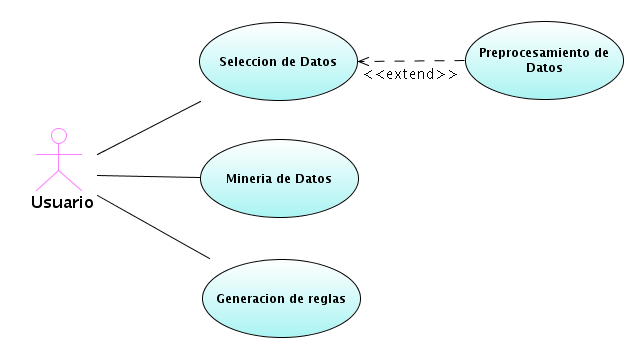
\includegraphics[width=0.9\textwidth]{imgsCasosUso/01tariy.png}
 \caption{Diagrama de caso de uso Tariy}
\end{figure}
\newpage

\subsubsection{M\'odulo de Selecci\'on}
\begin{figure}[h]
 \centering
 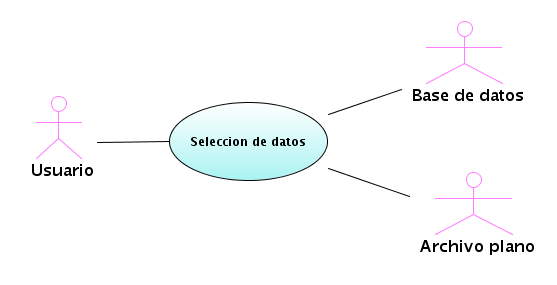
\includegraphics[width=0.9\textwidth]{imgsCasosUso/02seleccion.png}
 \caption{M\'odulo de Selecci\'on}
\end{figure}

\subsubsection{M\'odulo de Conexi\'on a Base de Datos}
\begin{figure}[h]
 \centering
 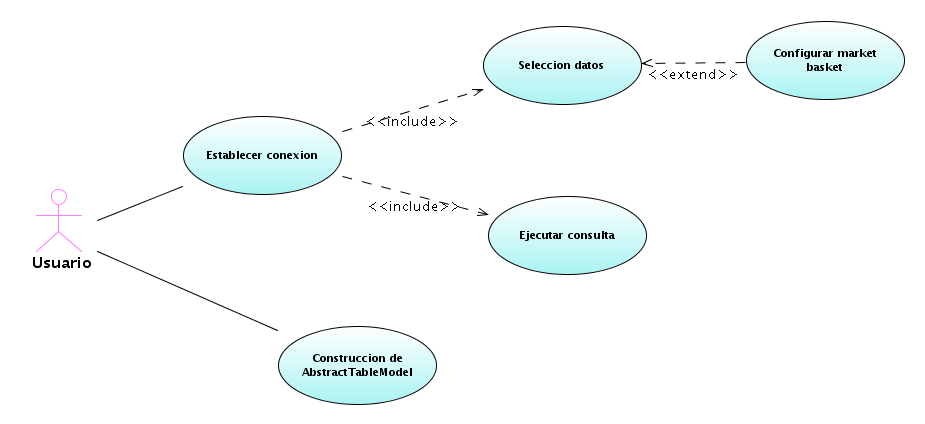
\includegraphics[width=0.9\textwidth]{imgsCasosUso/04conexionBD.png}
 \caption{Base de Datos}
\end{figure}
\newpage

\subsubsection{M\'odulo de Conexi\'on a Archivo Plano}
\begin{figure}[h]
 \centering
 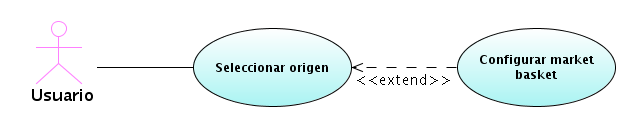
\includegraphics[width=0.9\textwidth]{imgsCasosUso/03archivoPlano.png}
 \caption{Archivo Plano}
\end{figure}

\subsubsection{M\'odulo de Preprocesamiento}
\begin{figure}[h]
 \centering
 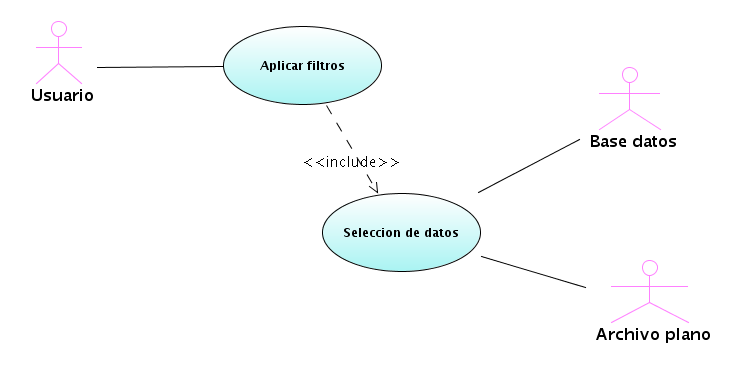
\includegraphics[width=0.9\textwidth]{imgsCasosUso/05preprocesamiento.png}
 \caption{Preprocesamiento}
\end{figure}
\newpage

\subsubsection{M\'odulo de Miner\'ia de Datos}
\begin{figure}[h]
 \centering
 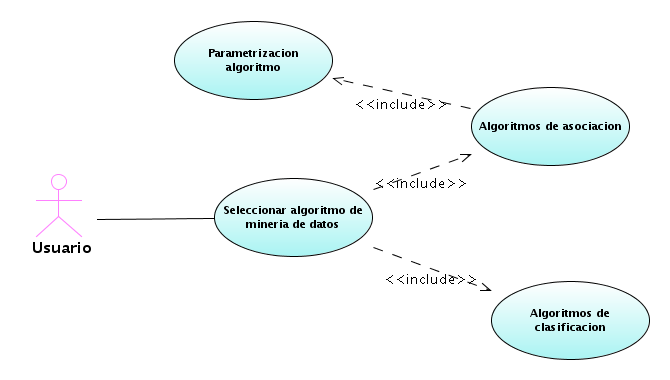
\includegraphics[width=0.9\textwidth]{imgsCasosUso/06mineria.png}
 \caption{Miner\'ia de Datos}
\end{figure}
\newpage

\subsubsection{M\'odulo de Reglas}
\begin{figure}[h]
 \centering
 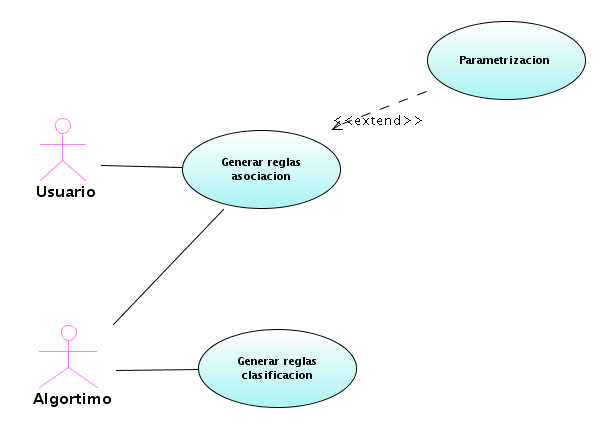
\includegraphics[width=0.9\textwidth]{imgsCasosUso/07reglas.png}
 \caption{Reglas}
\end{figure}
\newpage

%%%%%%%%%%%%%%%%%%%%%%%%%%% CLASE APRIORI %%%%%%%%%%%%%%%%%%%%%%%%%%%%%%%%%%%%%%%%%%%
\begin{figure}
\subsection{Diagramas de Secuencia}
\subsubsection{Clase Apriori}
\centering
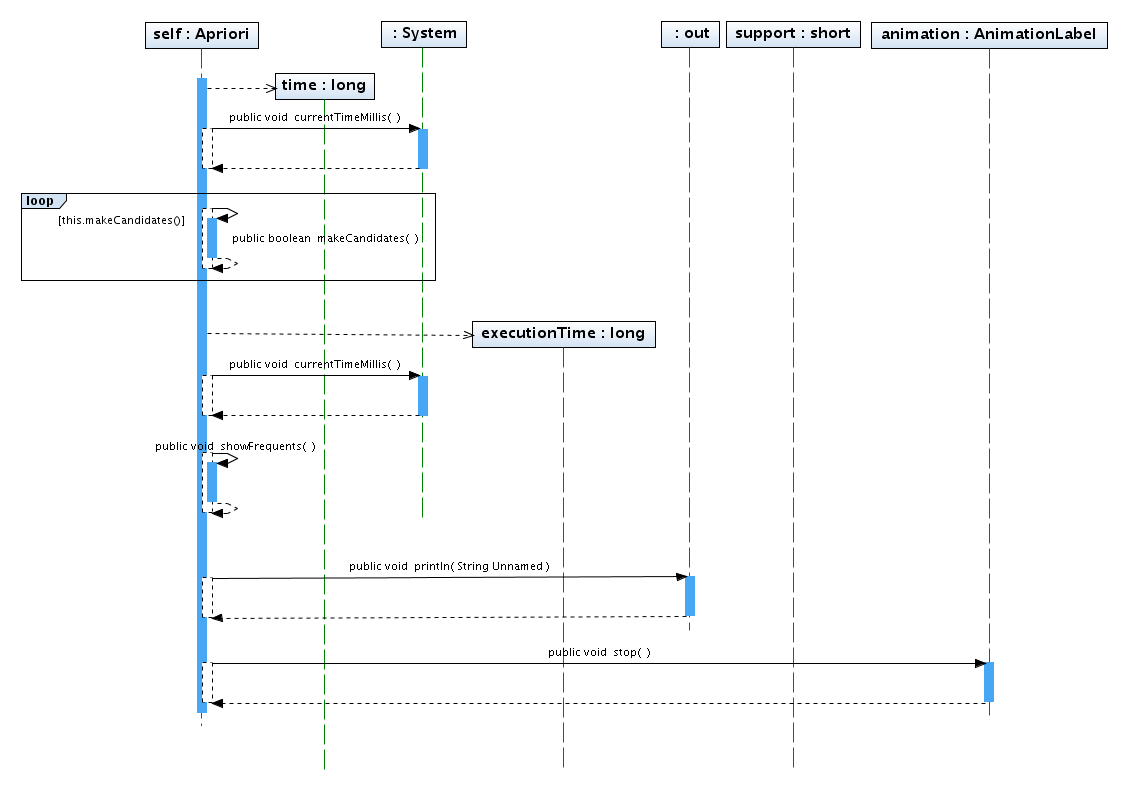
\includegraphics[width=1.2\textwidth]{imgsSecuencia/Apriori/run.png}
\caption{run}
\end{figure}
\newpage
\begin{figure}
\centering
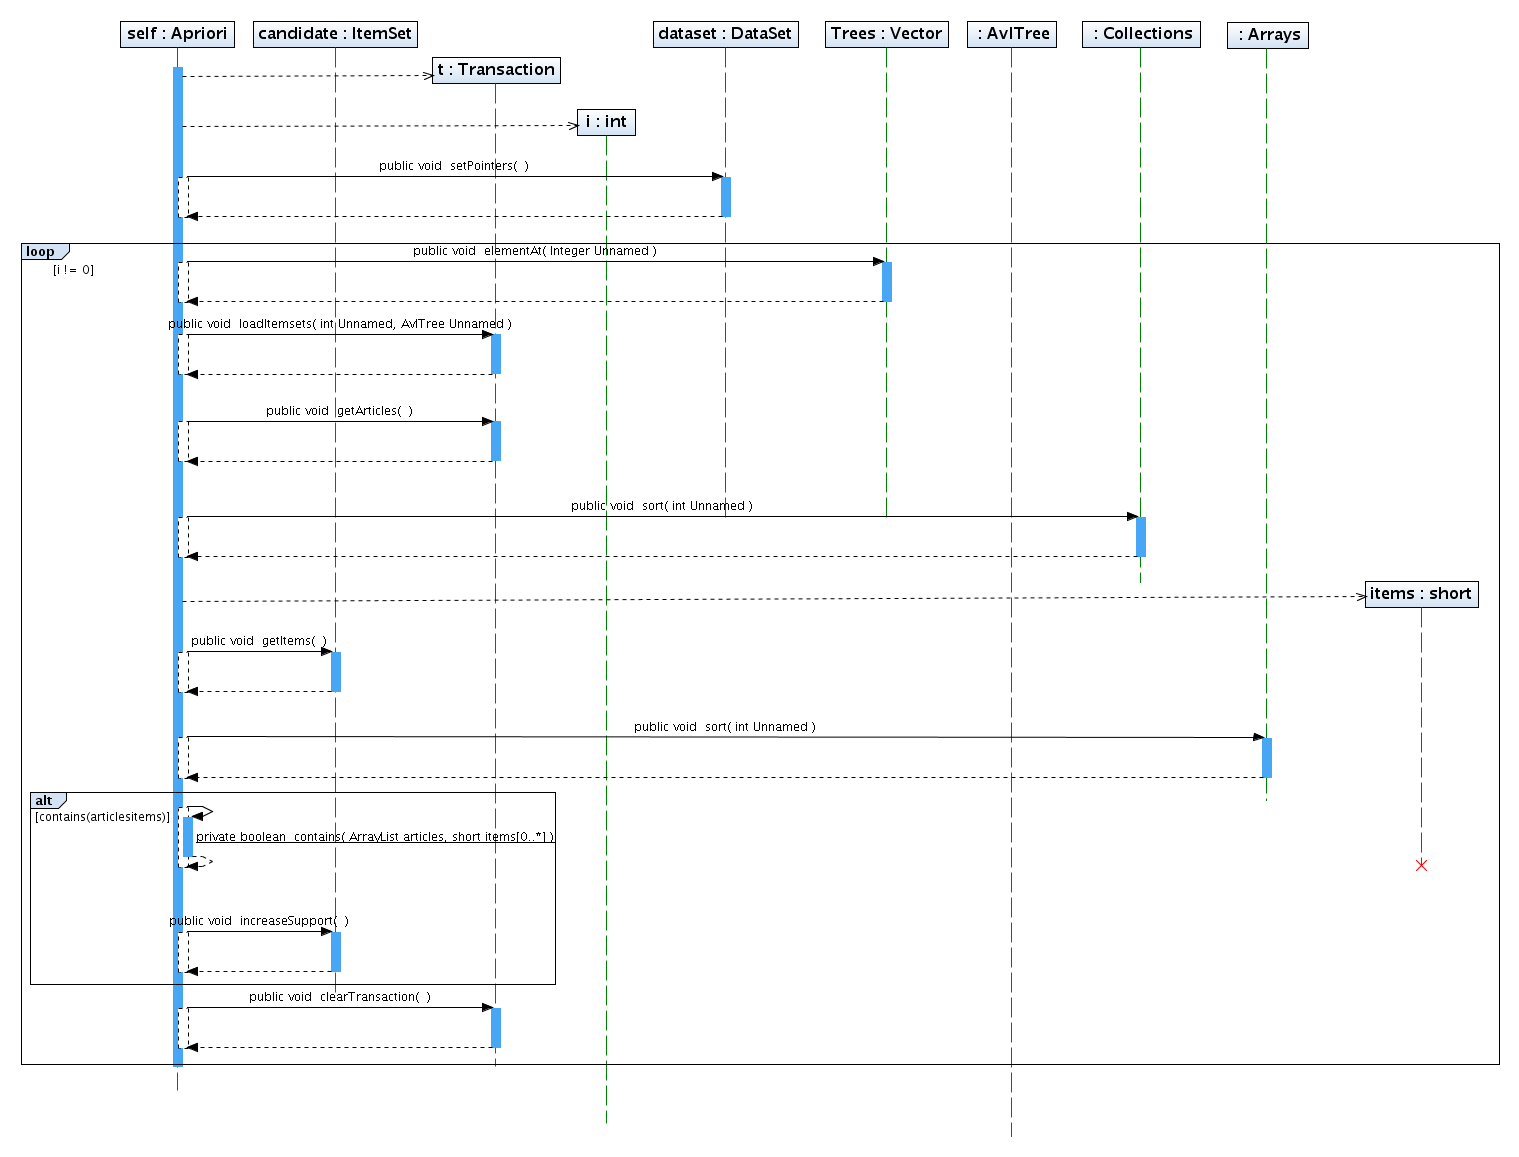
\includegraphics[width=1.2\textwidth]{imgsSecuencia/Apriori/increaseSupport.png}
\caption{increaseSupport}
\end{figure}
\newpage
\begin{figure}
\centering
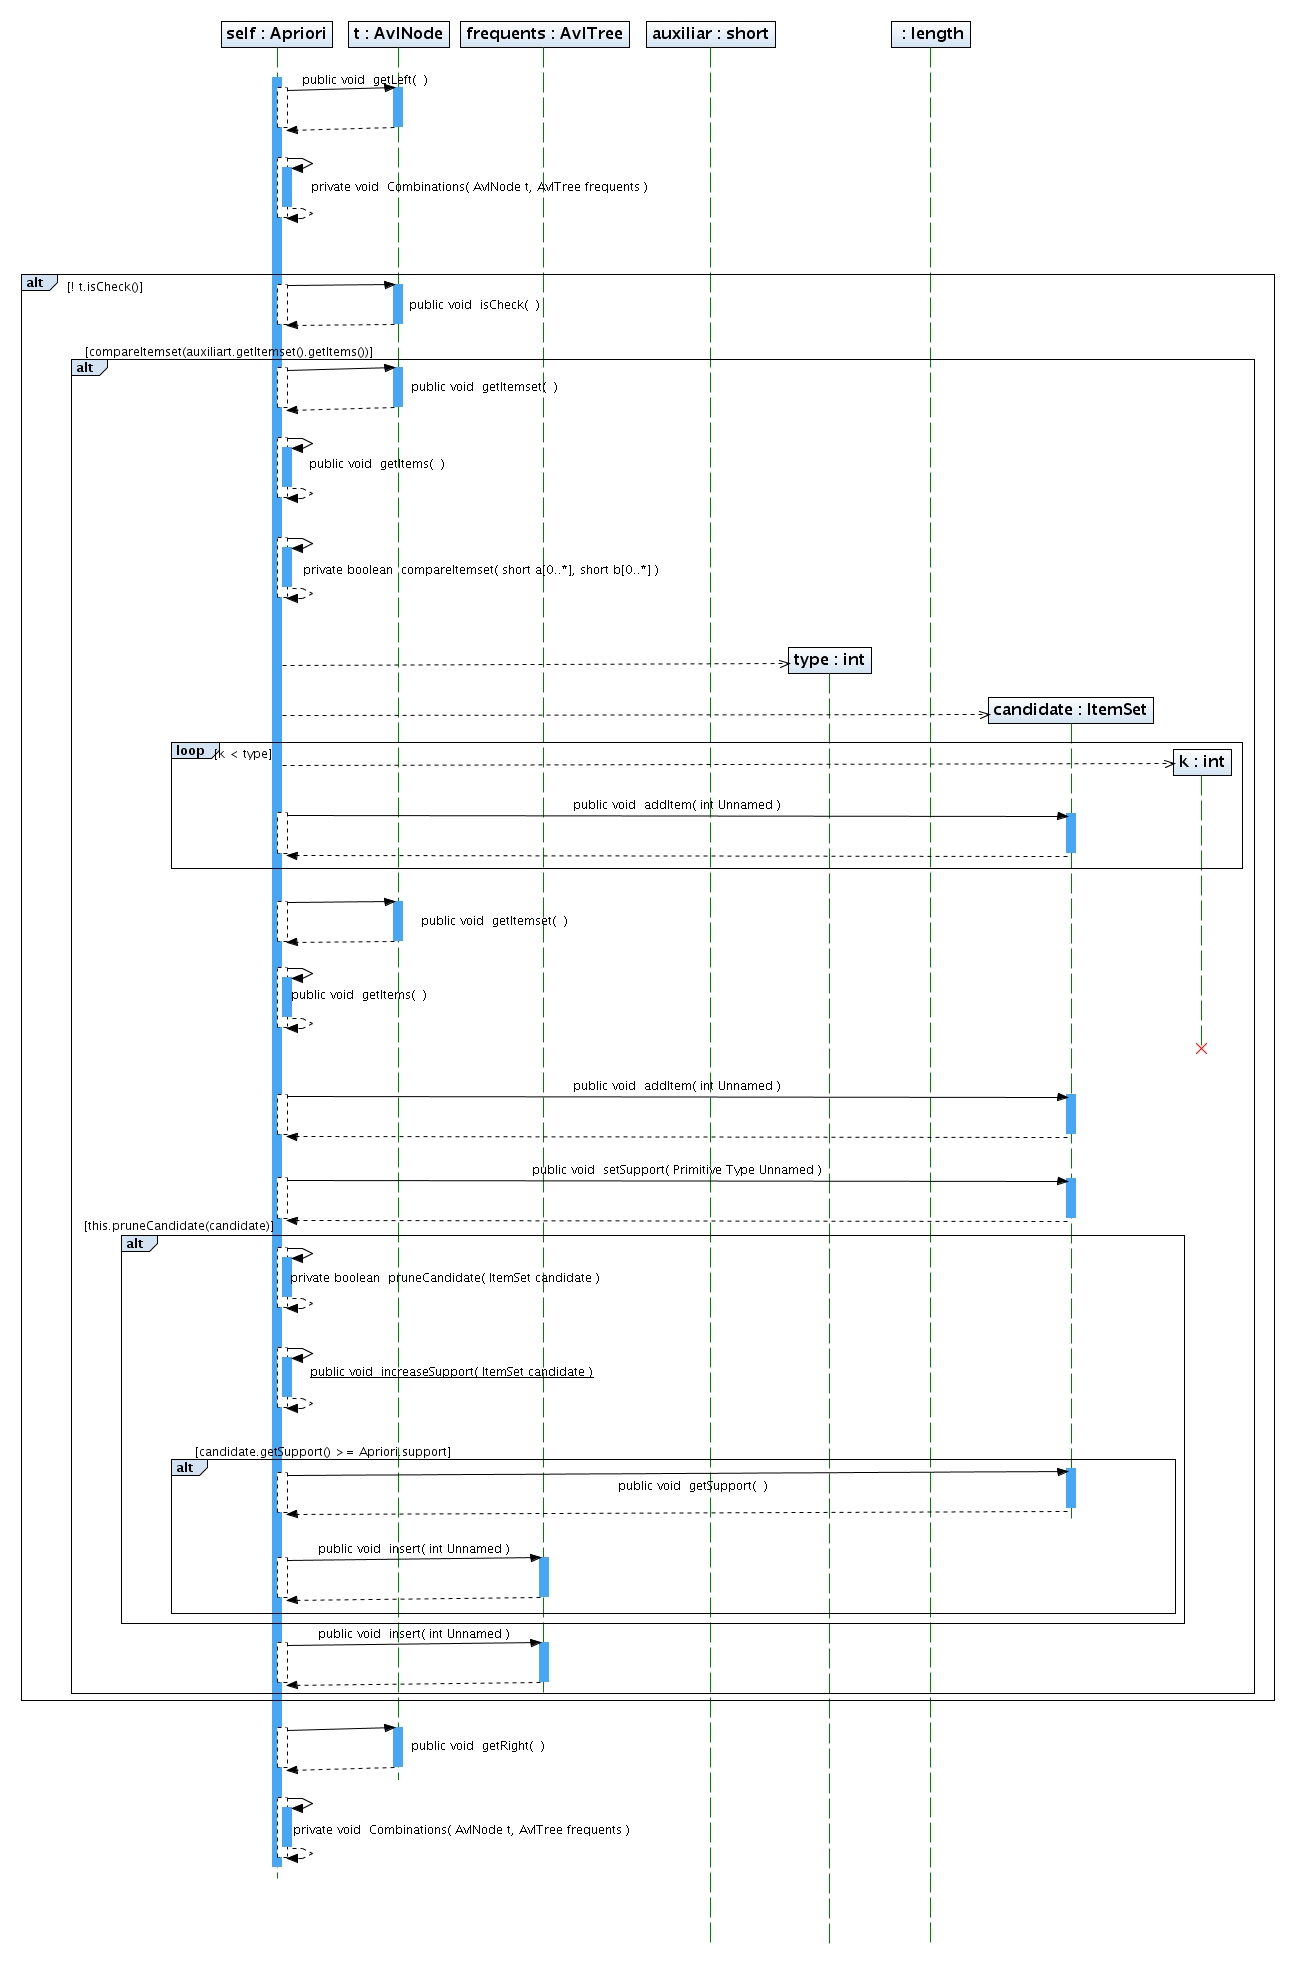
\includegraphics[width=0.8\textwidth]{imgsSecuencia/Apriori/CombinationsB.jpg}
\caption{Combinations}
\end{figure}
\newpage
\begin{figure}
\centering
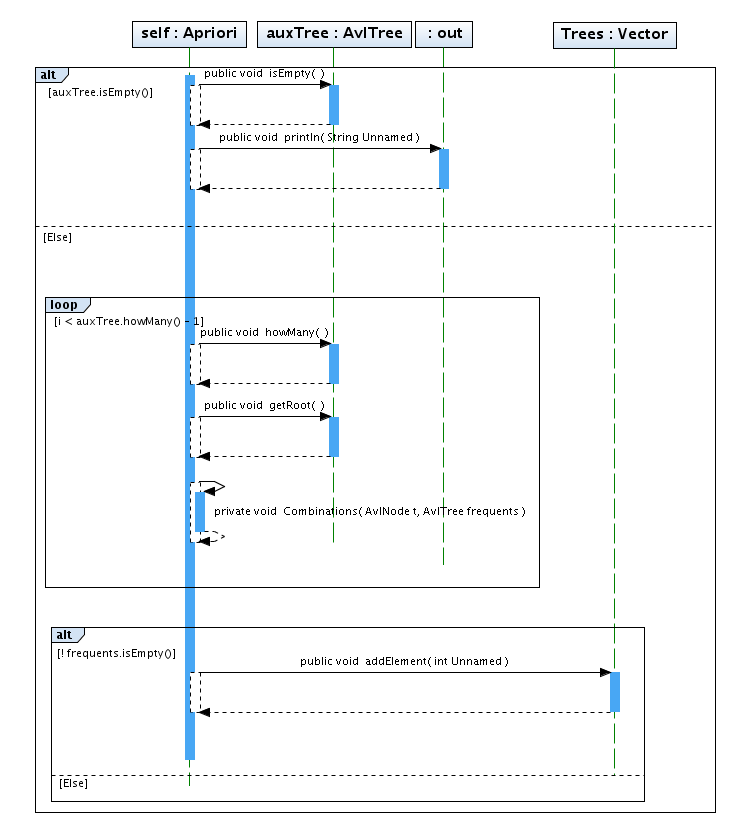
\includegraphics[width=1\textwidth]{imgsSecuencia/Apriori/makeCandidates.png}
\caption{makeCandidates}
\end{figure}
\newpage
\begin{figure}
\centering
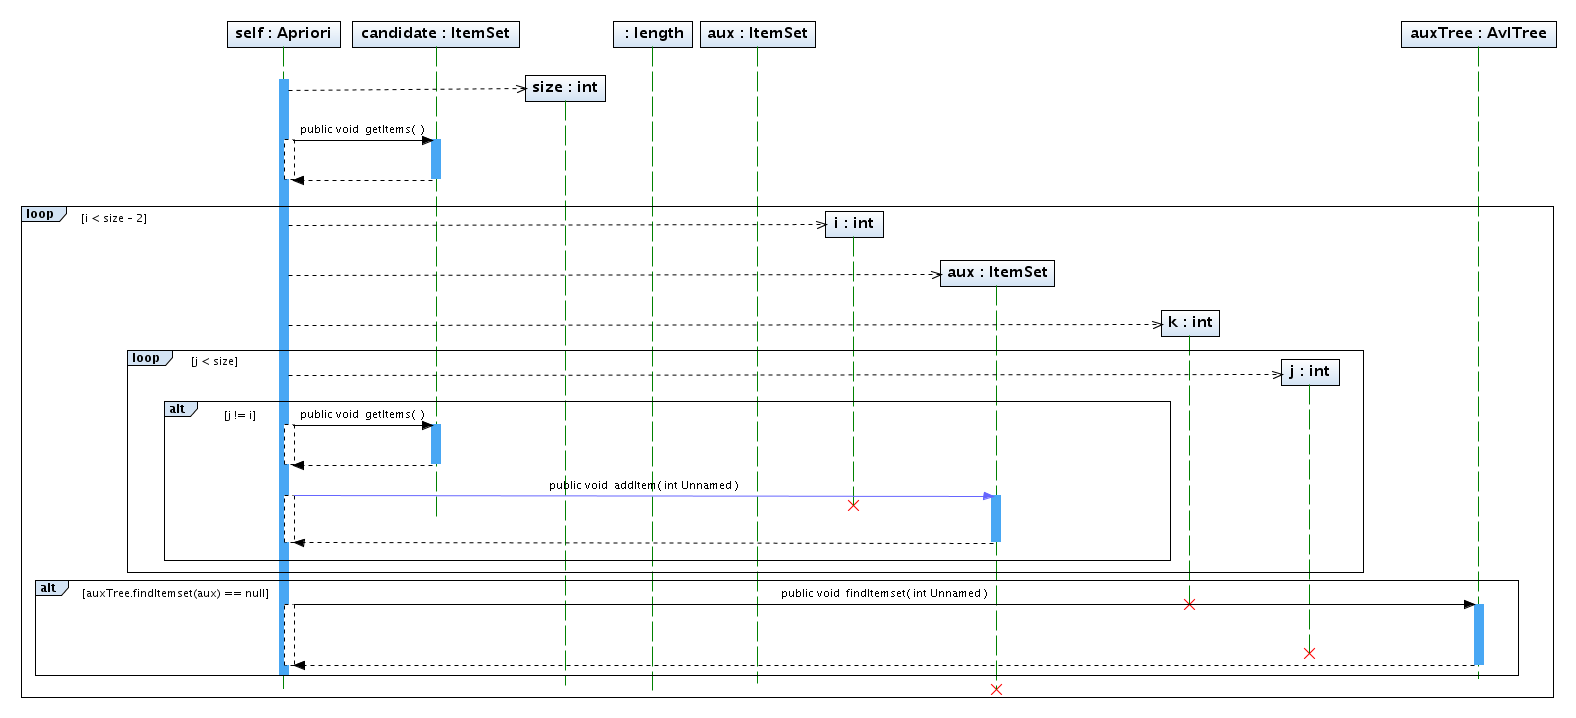
\includegraphics[angle=90, width=0.5\textwidth]{imgsSecuencia/Apriori/pruneCandidates.png}
\caption{pruneCandidates}
\end{figure}
\newpage

%%%%%%%%%%%%%%%%%%%%%%%%%% CLASE EQUIPASSO %%%%%%%%%%%%%%%%%%%%%%%%%%%%%%%%%%%%%%%%%%%%
\begin{figure}
\subsubsection{Clase EquipAsso}
\centering
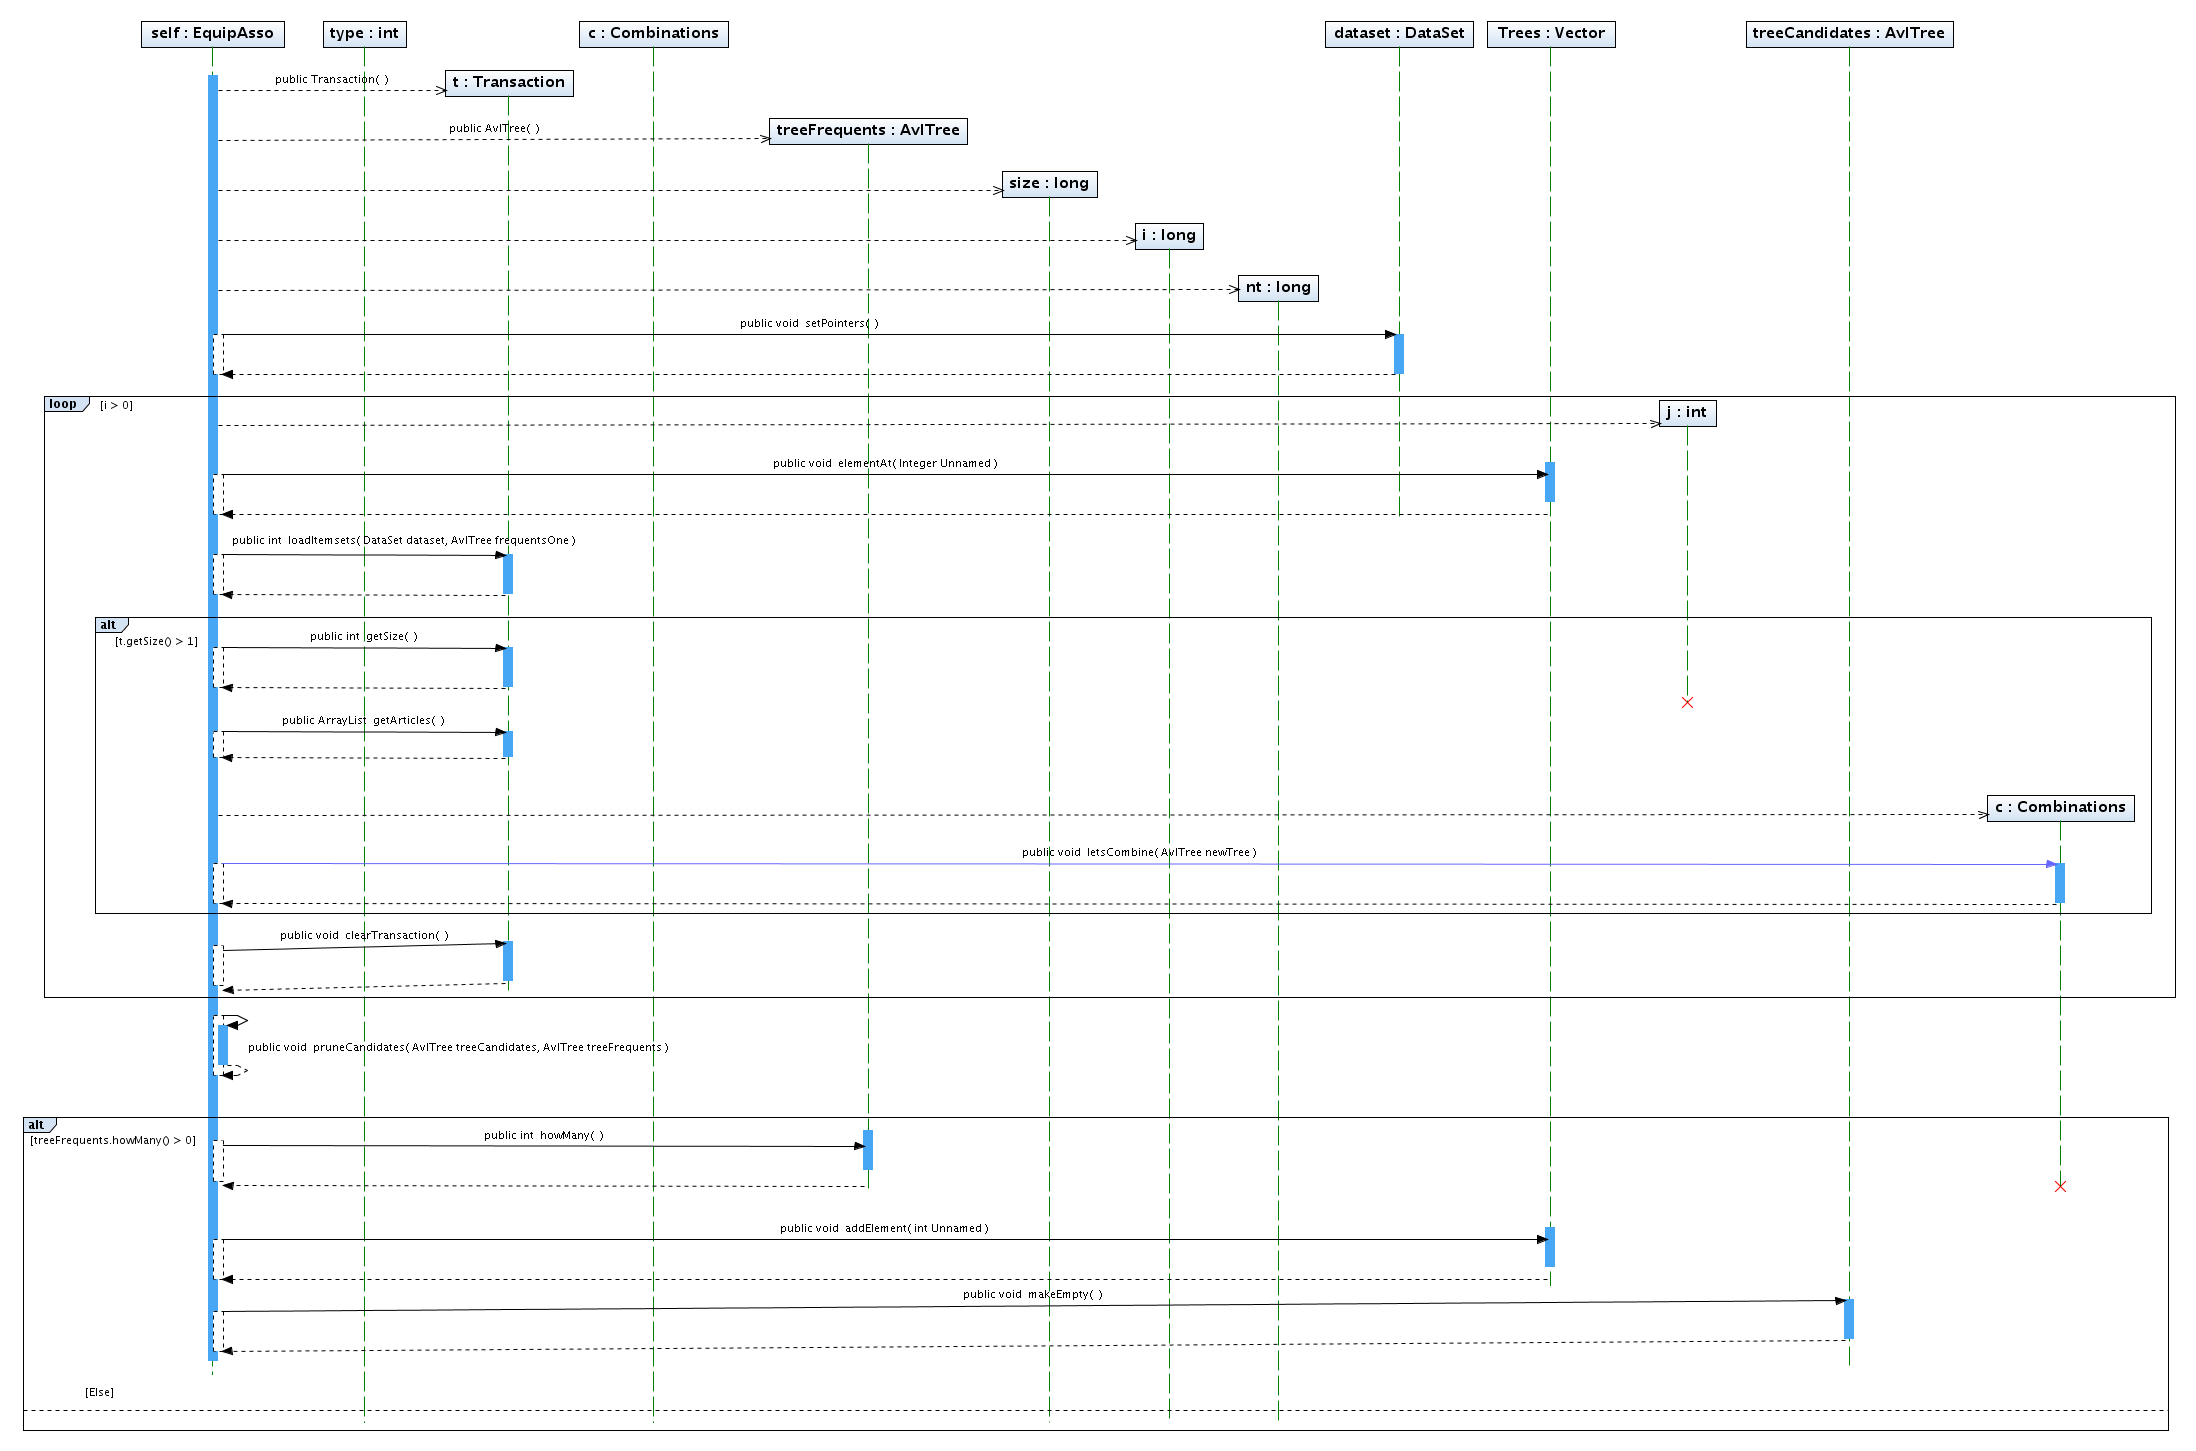
\includegraphics[angle=90, width=0.8\textwidth]{imgsSecuencia/EquipAsso/findInDataSet.png}
\caption{findInDataSet}
\end{figure}
\newpage
\begin{figure}
\centering
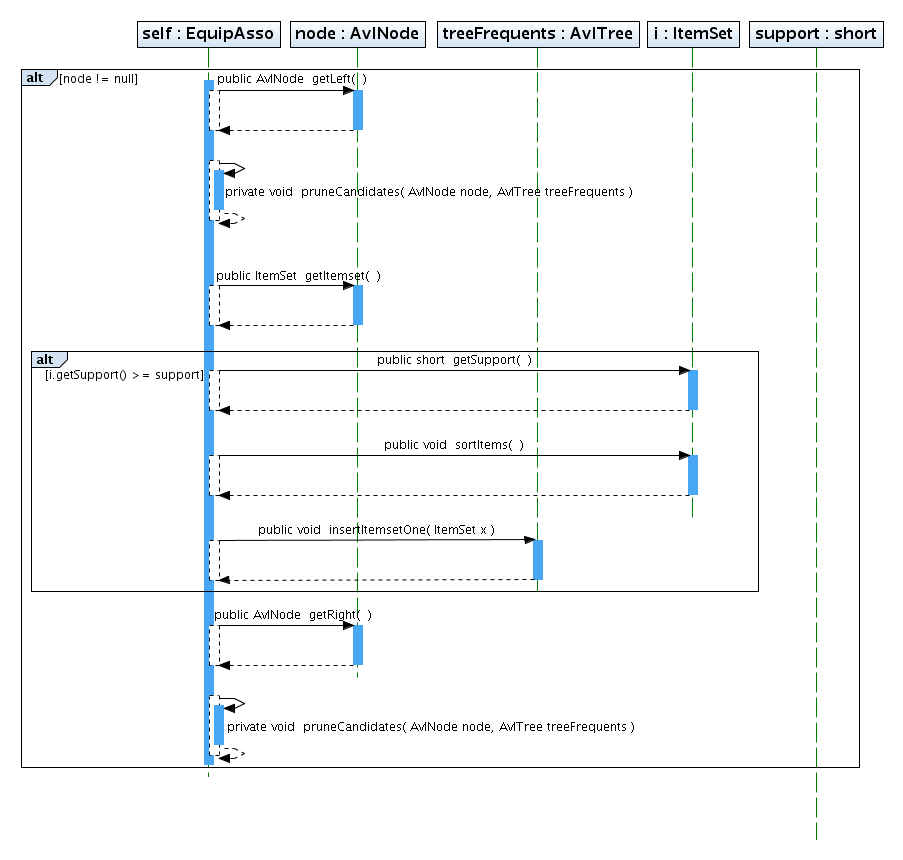
\includegraphics[width=0.8\textwidth]{imgsSecuencia/EquipAsso/pruneCandidate-recursive.png}
\caption{pruneCandidate-recursive}
\end{figure}
\newpage
\begin{figure}
\centering
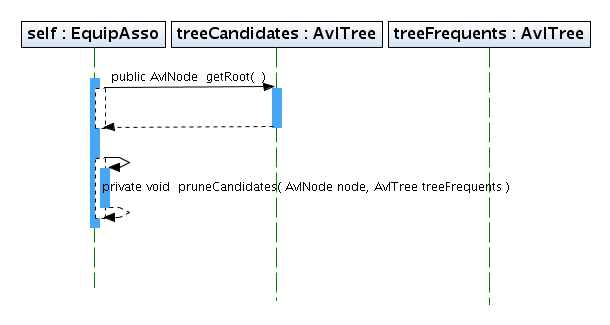
\includegraphics[width=1.2\textwidth]{imgsSecuencia/EquipAsso/pruneCandidates.png}
\caption{pruneCandidate-recursive}
\end{figure}
\newpage
\begin{figure}
\centering
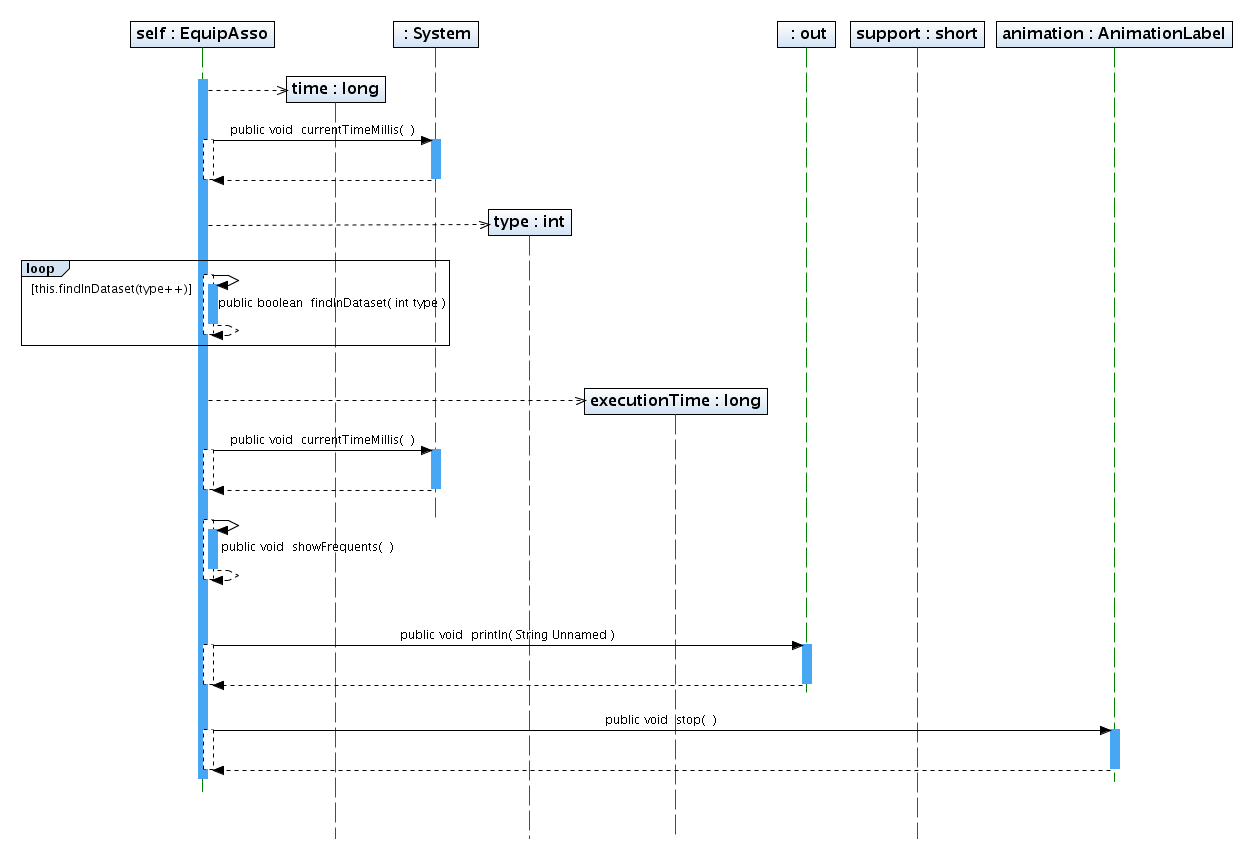
\includegraphics[width=1.2\textwidth]{imgsSecuencia/EquipAsso/run.png}
\caption{run}
\end{figure}
\newpage

%%%%%%%%%%%%%%%%%%%%%%%% CLASE ITEMSET %%%%%%%%%%%%%%%%%%%%%%%%%%%%%%%%%%%%%
\begin{figure}
\subsubsection{Clase ItemSet}
\centering
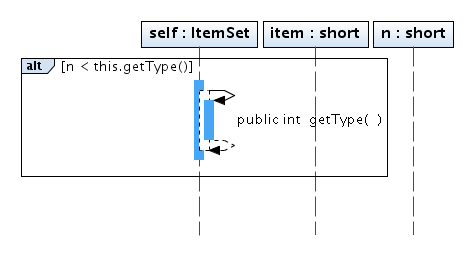
\includegraphics[width=0.7\textwidth]{imgsSecuencia/ItemSet/addItems.png}
\caption{addItems}
\end{figure}
\newpage
\begin{figure}
\centering
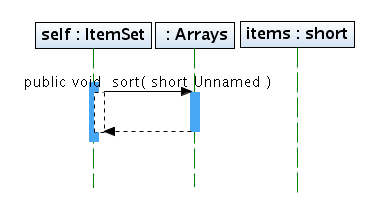
\includegraphics[width=0.7\textwidth]{imgsSecuencia/ItemSet/sortItems.png}
\caption{sortItems}
\end{figure}
\newpage
\begin{figure}
\centering
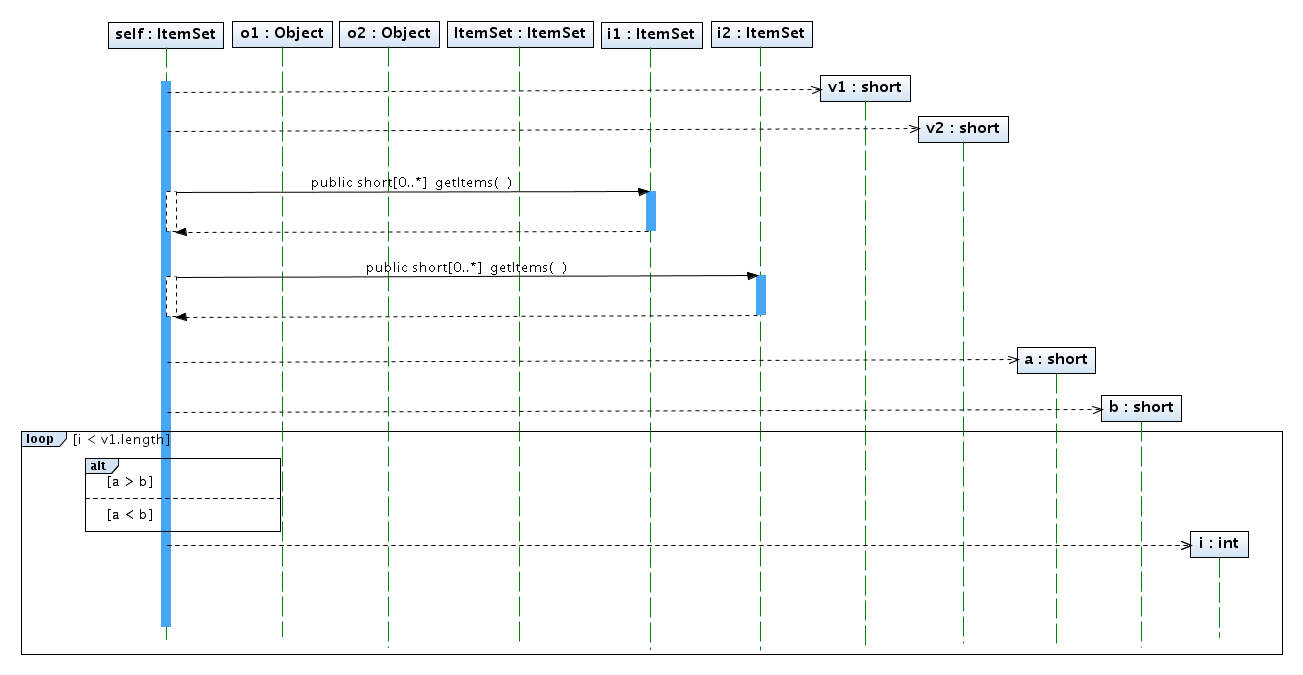
\includegraphics[angle=90, width=0.5\textwidth]{imgsSecuencia/ItemSet/compare.png}
\caption{compare}
\end{figure}
\newpage

%%%%%%%%%%%%%%%%%%%%%%%% CLASE DATASET %%%%%%%%%%%%%%%%%%%%%%%%%%%%%%%%%%%%%%%%%
\begin{figure}
\subsubsection{Clase DataSet}
\centering
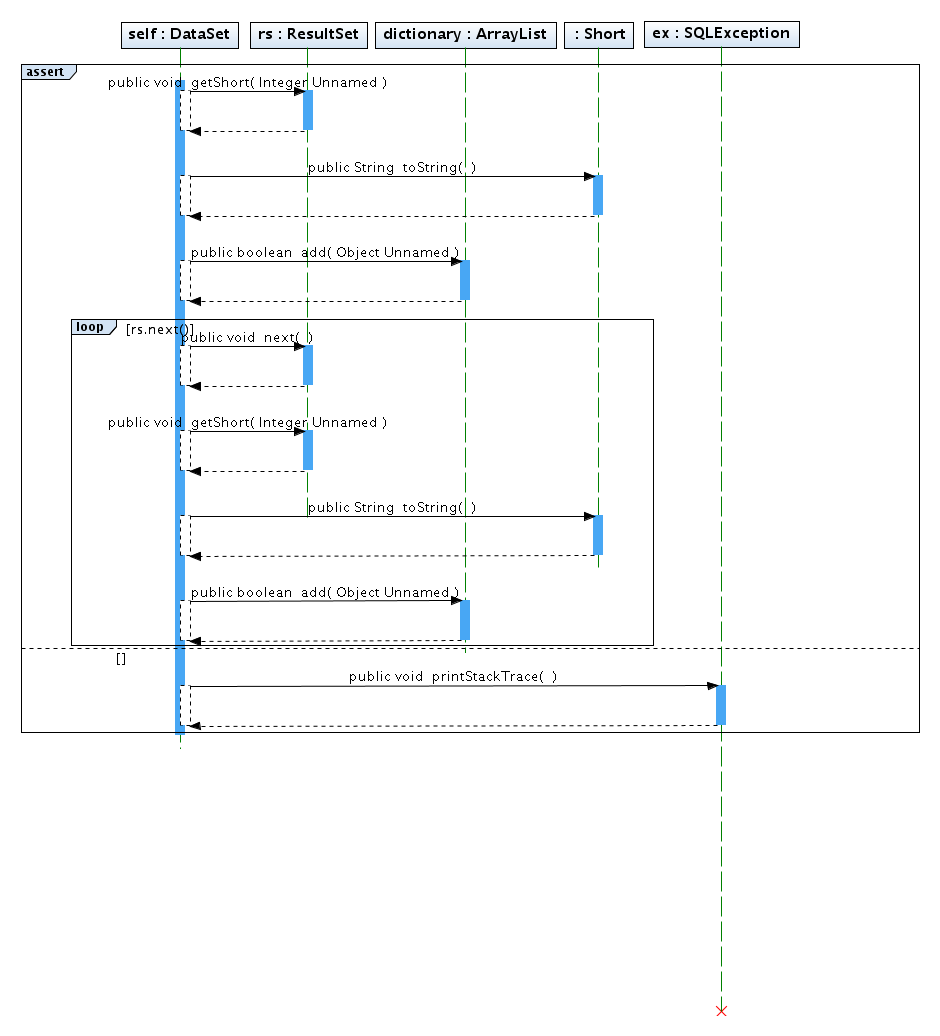
\includegraphics[width=1\textwidth]{imgsSecuencia/DataSet/buildDictionary.png}
\caption{buildDictionary}
\end{figure}
\newpage
\begin{figure}
\centering
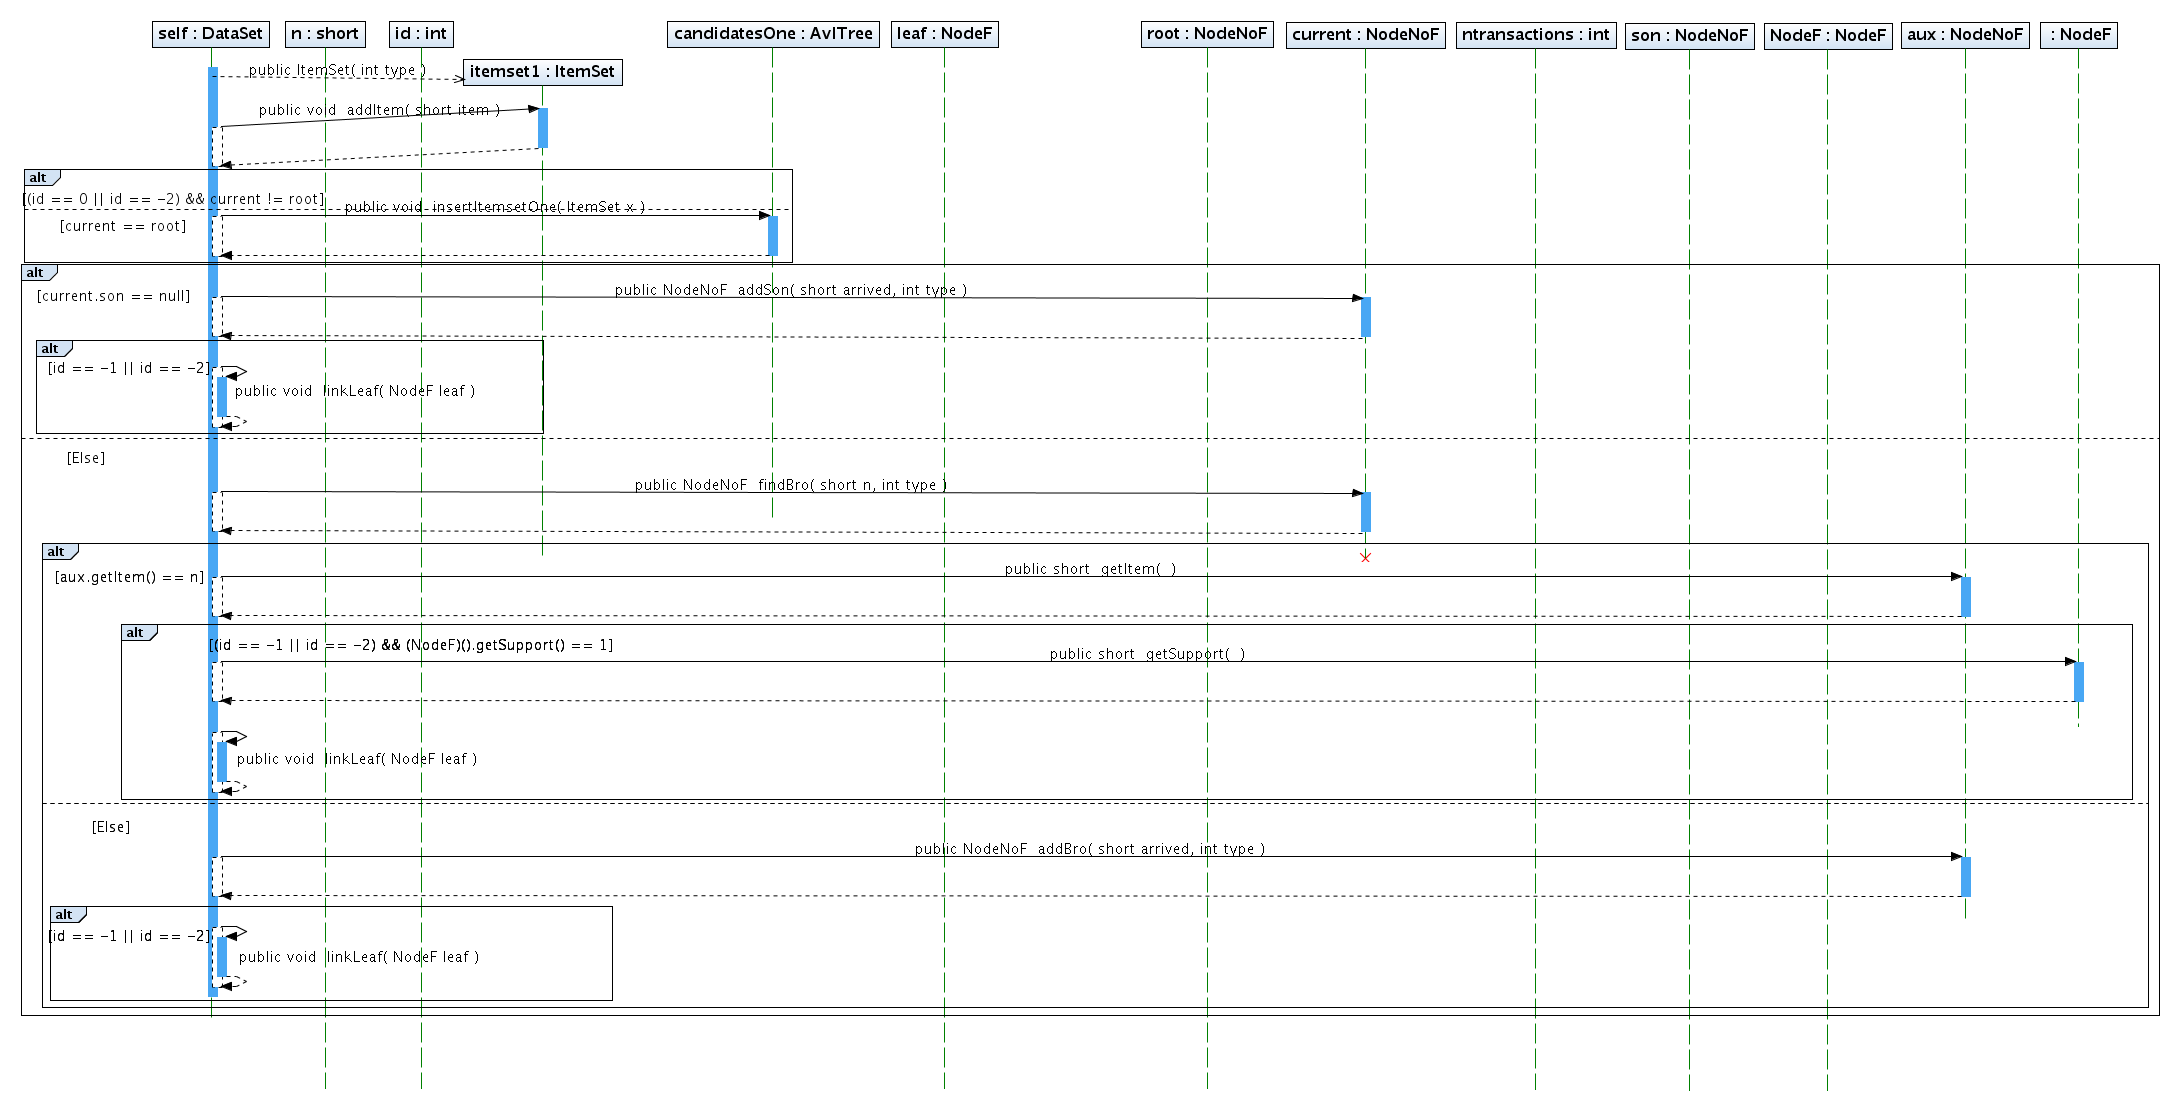
\includegraphics[angle=90, width=0.6\textwidth]{imgsSecuencia/DataSet/buildNTree.png}
\caption{buildNTree}
\end{figure}
\newpage
\begin{figure}
\centering
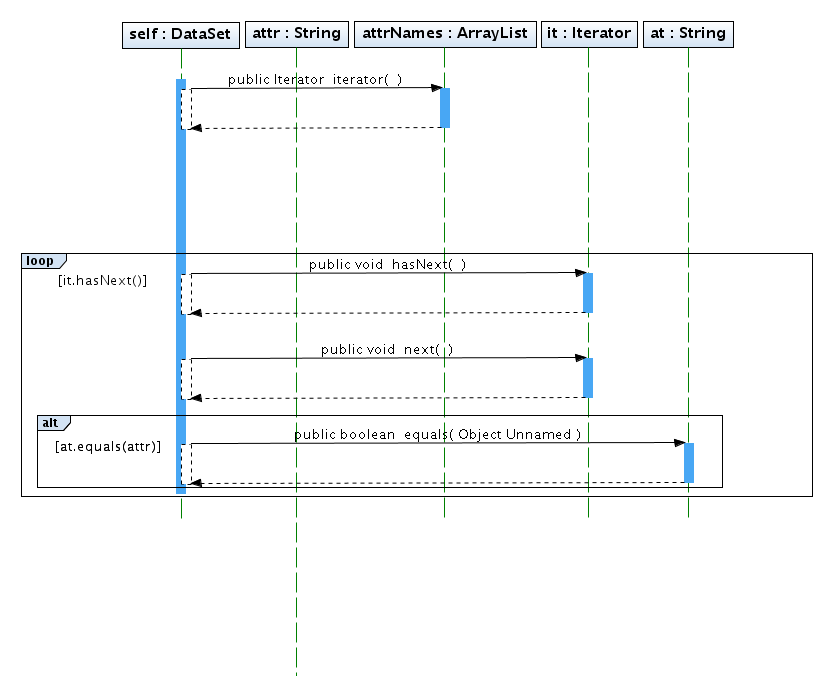
\includegraphics[width=1\textwidth]{imgsSecuencia/DataSet/findAttrName.png}
\caption{findAttrName}
\end{figure}
\newpage
\begin{figure}
\centering
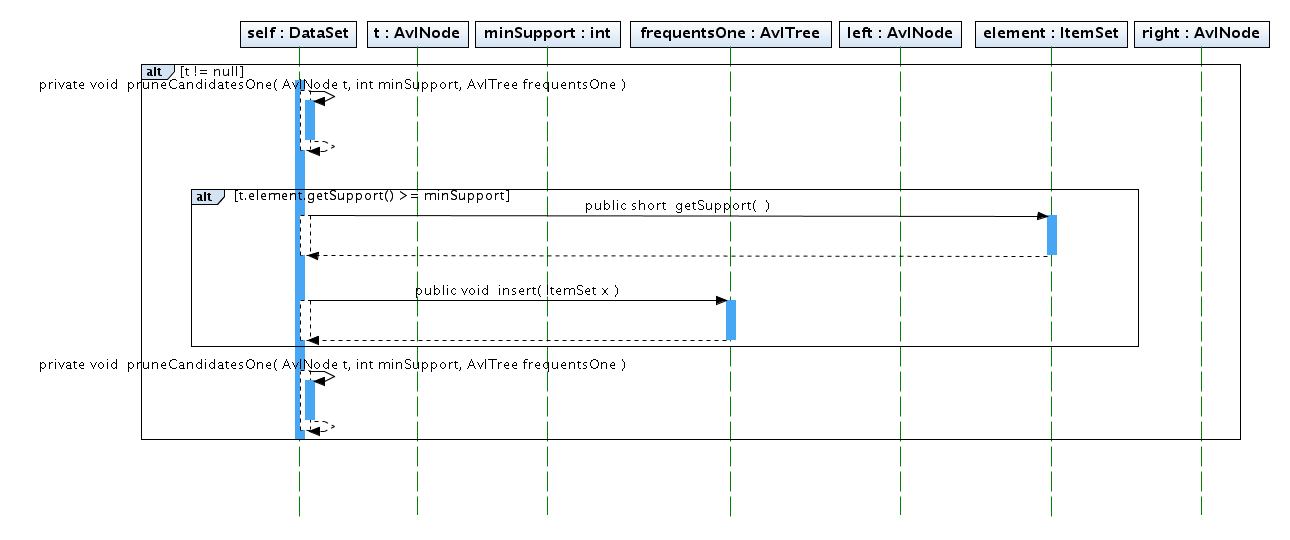
\includegraphics[angle=90, width=0.5\textwidth]{imgsSecuencia/DataSet/pruneCandidatesOne.png}
\caption{pruneCandidatesOne}
\end{figure}
\newpage
\begin{figure}
\centering
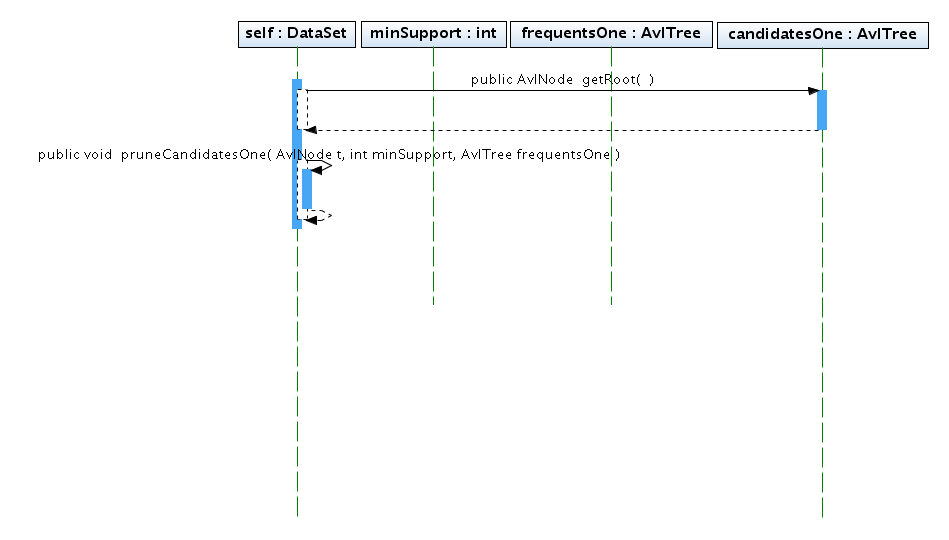
\includegraphics[width=1.2\textwidth]{imgsSecuencia/DataSet/pruneCandidatesOne_public.png}
\caption{public-pruneCandidatesOne}
\end{figure}
\newpage
